\documentclass[landscape,a0,final]{a0poster}
\usepackage[dvipsnames,svgnames]{xcolor}
\usepackage{tikzposter} % here most of the things are defined
% change parameters only after this line You can also start a new column with an arbitrary 
% x-coordinate by specifying explicitly the coordinate of the new block node as follows:
% needed for authors:
\usepackage[czech]{babel}
\usepackage[utf8]{inputenc}
\usepackage{wrapfig}
\usepackage{url}
\usepackage{alltt}
\usepackage{textcomp}

\usepackage[margin=\margin cm, paperwidth=197cm, paperheight=100cm]{geometry}

\usepackage{listings}

% \setbackgrounddarkcolor{ForestGreen!70!black}
% \setbackgroundlightcolor{YellowGreen!90!}

% \setfirstcolor{YellowGreen!80!}
% \setsecondcolor{gray!80!}
% \setthirdcolor{red!80!black}

\title{\bigskip GRASS GIS Vector State of the Art  --  Gearing towards GRASS GIS 7 \bigskip}
\author{Markus Metz$^1$, Martin Landa$^2$, Anna Petrášova$^3$, Vaclav Petráš$^3$, Yann Chemin$^4$, Markus Neteler$^1$ and The GRASS GIS Development Team\\ \bigskip
$^1$ CRI, FEM, Italy, $^2$ CTU in Prague, Czech Republic, $^3$ NCSU, USA, $^4$ IWMI, Sri Lanka}

\usetemplate{1}
\setinstituteshift{1}

\setblocktitleheight{2}
\setblockspacing{1}

\begin{document}
\ClearShipoutPicture
\AddToShipoutPicture{\BackgroundPicture}
\noindent
\tikzstyle{every picture}+=[remember picture]
\begin{tikzpicture}
\initializesizeandshifts
\titleblock{123.8}{1}
% \setblocktitleheight{1}

\addlogo[north west]{(2,-1)}{9cm}{svg_images/Grass_GIS.pdf}
%Please insert your institution logo here
\addlogo[north east]{(-2,-2.5)}{4cm}{svg_images/logo_FEM_CRI.pdf}
\addlogo[north east]{(-2,-5.5)}{4cm}{svg_images/NC_State_Seal.pdf}
\addlogo[north east]{(-8,-2.5)}{4cm}{images/Logo_cvut.jpg}
\addlogo[north east]{(-8,-6.5)}{4cm}{svg_images/IWMI_logo.pdf}

%%%%%%%%%%%%%%%%%%%%%%%%%%%%%%%%%%%%%%%%%%%%%%%%%%%%%%%%%%%%%%%%%%%%%%%%%%%%%%%%
\blocknode{Abstract}{
% \small <<- too small for a poster!
The upcoming GRASS GIS 7 release improves not only raster processing and general design but the vector processing in the first place. GRASS GIS, as a topological GIS, recognizes that the topology plays the key role in the vector processing and analysis.\newline
Topology ensures that adjacent geographic components in a single vector map are related. In contrast to non-topological GIS, a border common to two areas exists only once and is shared between the two areas. Topological representation of vector data helps to produce and maintain vector maps with clean geometry as well as enables the user to perform certain analyses that can not be conducted with non-topological or spaghetti data. Non-topological vector data are automatically converted to a topological representation upon import. Further more, various cleaning tools exist to remove non-trivial topological errors.\newline
In the upcoming GRASS GIS 7 release the vector library was particularly improved to make it faster and more efficient with an improved internal vector file format. This new topological format reduces memory and disk space requirements, leading to a generally faster processing. Opening an existing vector requires less memory providing additionally support for large files. The new spatial index performs queries faster (compared to GRASS GIS 6 more than 10 times for large vectors). As a new option the user can select a file-based version of the spatial index for large vector data. All topological cleaning tools have been optimized with regard to processing speed, robustness, and system requirements.\newline
The vector engine comes with a new prototype for direct read/write support of OGR Simple Features API.\newline
Additionally vector data can be directly exchanged with topological PostGIS 2 databases. This enables GRASS to read and write topological primitives beside native file-based format also to the topological PostGIS 2 databases. \newline
Considering the wide spread usage of Esri Shapefile, a non-topological format for vector data exchange, it is particularly advantageous that GRASS GIS 7 offers advanced cleaning tools.\newline
For power users and programmers, the new Python interface allows to directly access functions provided by the underlying C libraries; this combines the ease of writing Python scripts with the power of optimized C functionality in the library backend.
}

%%%%%%%%%%%%%%%%%%%%%%%%%%%%%%%%%%%%%%%%%%%%%%%%%%%%%%%%%%%%%%%%%%%%%%%%%%%%%%%%
\blocknode{Topology support}{
\small
The GRASS GIS native vector format stores objects in a topology format. The OGC Simple Features can be imported into and exported from the GRASS GIS format through topological vector conversion. For attribute management several database management system (DBMS) with SQL support are supported including SQLite (default DB backend), DBF, PostgreSQL, MySQL, ODBC.

The following \textbf{basic topological elements} can be edited directly: point, centroid, line, and boundary. A GRASS vector map can contain a~combination of several different types of the elements.
From these basic geometry types the following \textbf{derived topological elements} can be generated: area (closed ring of boundaries + centroid), isle (closed ring of boundaries, no centroid), and node (at both ends of lines/boundaries). Isles and Nodes are not visible to the user. Furthermore face, kernel (3D centroid) and volume (3D area) as defined in the format.

% TODO: point to http://grass.osgeo.org/programming7/

% TODO: 2. explain topology changes <<- needed?


% TODO: show the internal format change or rather the actual model?
\begin{center}
 \includegraphics[width=0.48\textwidth]{odp_slides/grass7_basic_vector_types_digitizer}
 \hspace{10mm}
 \includegraphics[width=0.48\textwidth]{odp_slides/grass7_derived_vector_types}
 \newline
 Figure 1a: Basic and derived topological elements in GRASS GIS 7
\end{center}

\begin{center}
 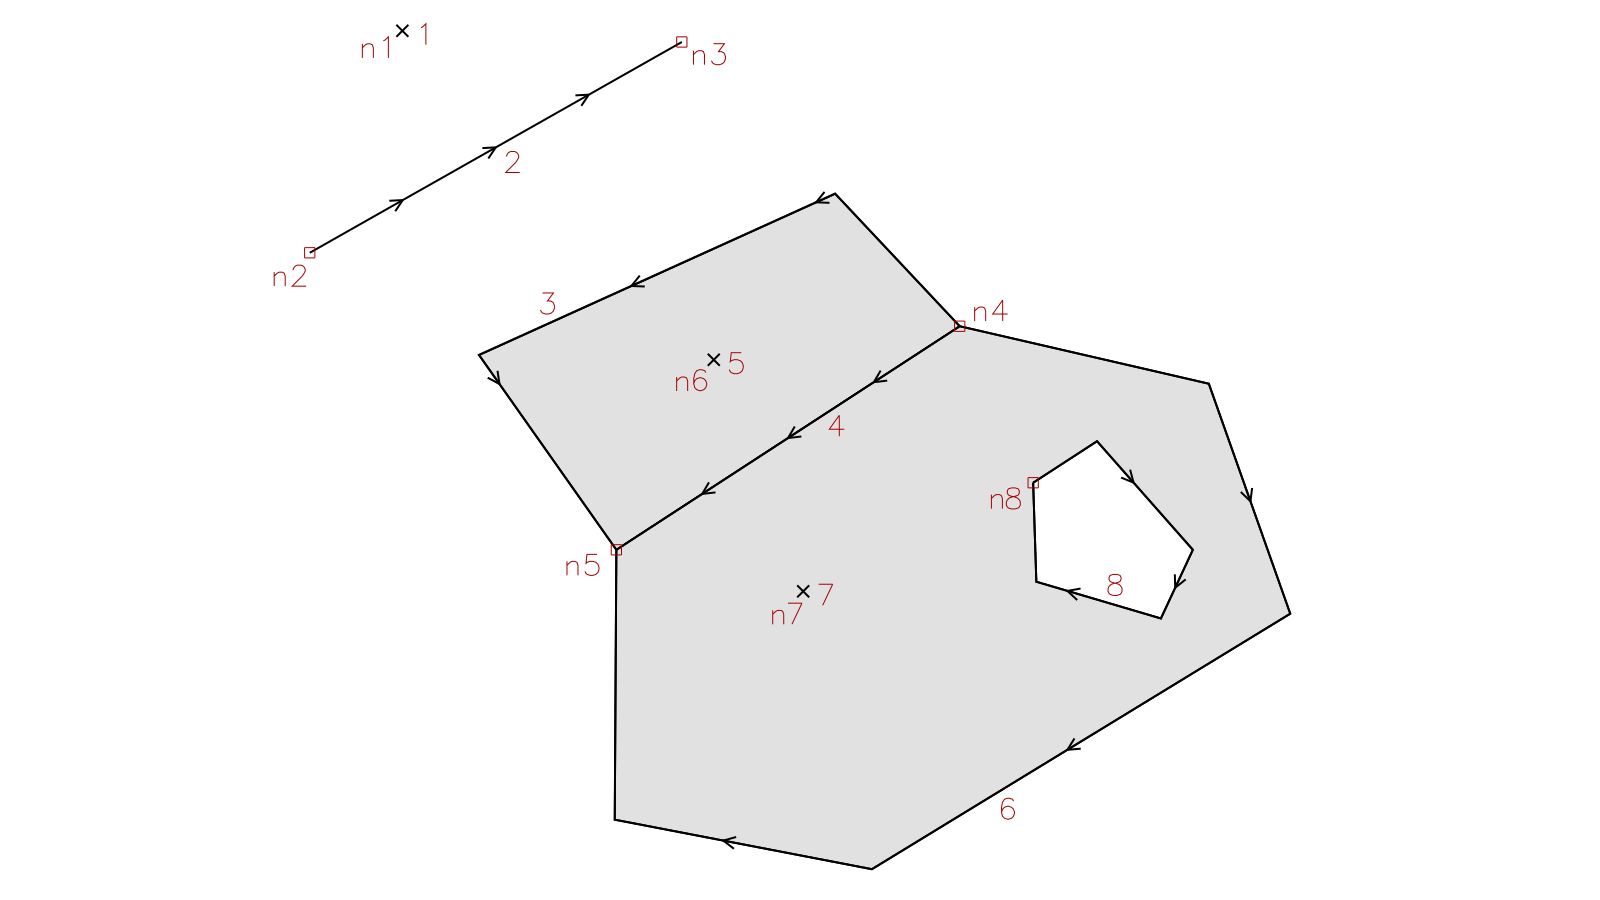
\includegraphics[width=0.38\textwidth]{svg_images/grass6-topo}
 \hspace{10mm}
 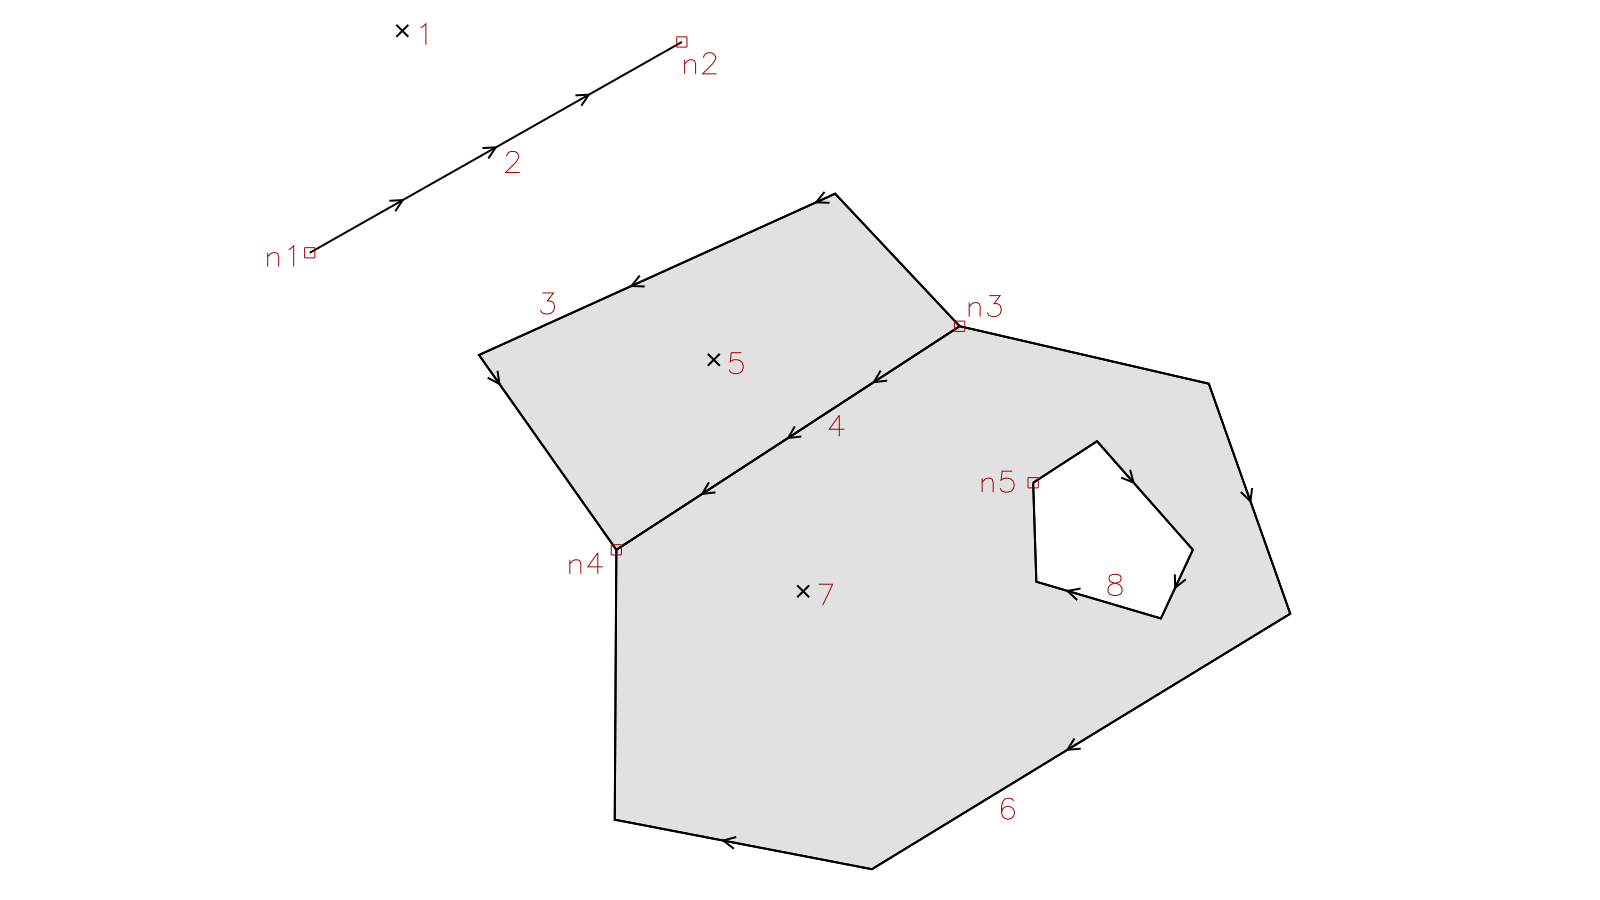
\includegraphics[width=0.38\textwidth]{svg_images/grass7-topo}
 \newline
 Figure 1b: Topology changes from version 6 to 7 after (points and centroids are represented by the nodes) [Landa 2013]
\end{center}
}

% ref was here, moved to last column

\startsecondcolumn

%%%%%%%%%%%%%%%%%%%%%%%%%%%%%%%%%%%%%%%%%%%%%%%%%%%%%%%%%%%%%%%%%%%%%%%%%%%%%%%%
\blocknode{Data Sources}{
This
\begin{center}
 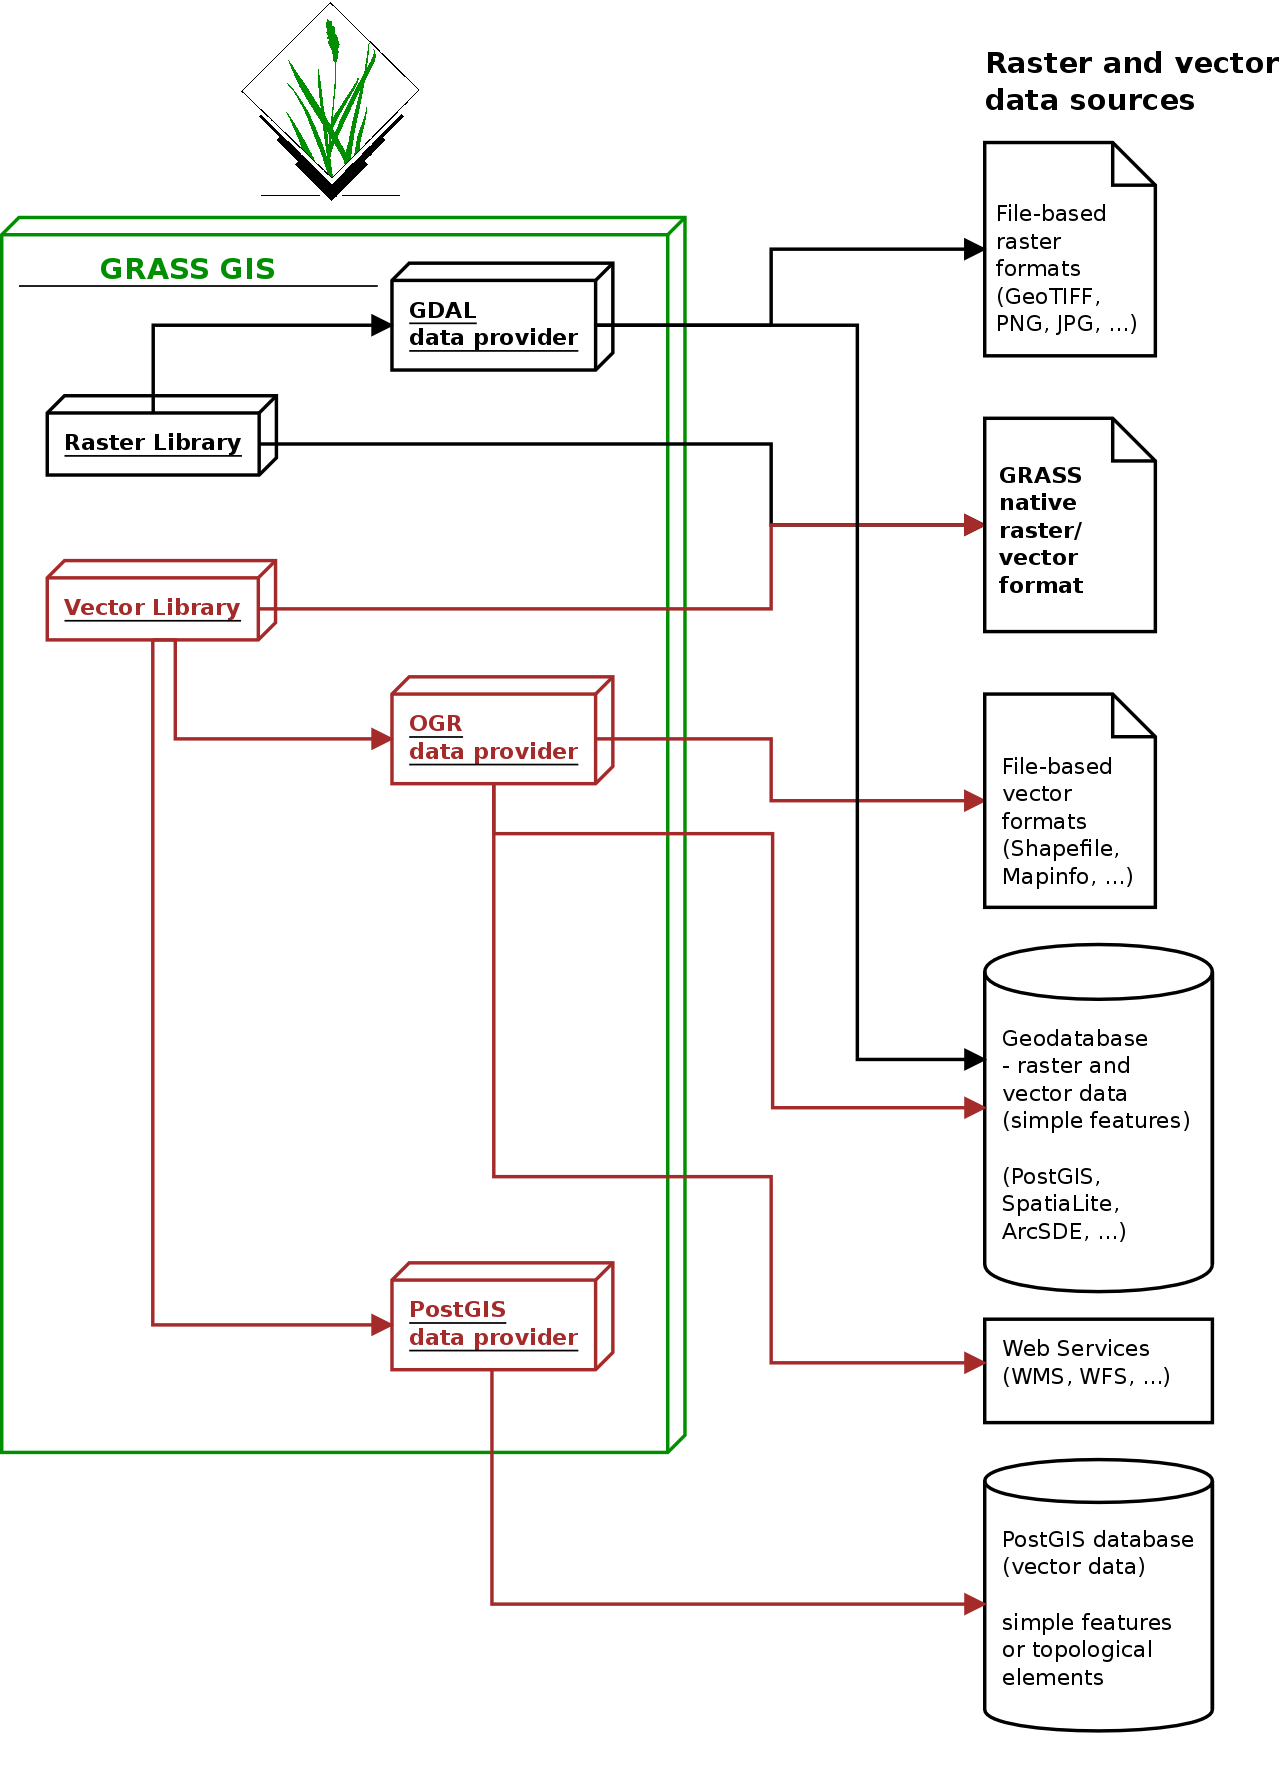
\includegraphics[width=0.47\textwidth]{images/grass-data-sources}
  \newline
 Figure 2: Data sources
\end{center}
}

%%%%%%%%%%%%%%%%%%%%%%%%%%%%%%%%%%%%%%%%%%%%%%%%%%%%%%%%%%%%%%%%%%%%%%%%%%%%%%%%
\blocknode{PyGRASS: fast Python API}{
PyGRASS [Zambelli 2013] is an object-oriented Python API which allows efficient manipulation with GRASS rasters and vectors.
It is easy-to-use but its performance is comparable to C code since it calls GRASS C API behind the scenes.

\includegraphics[width=0.9\textwidth]{texpdfs/pygrass_code}

}

%%%%%%%%%%%%%%%%%%%%%%%%%%%%%%%%%%%%%%%%%%%%%%%%%%%%%%%%%%%%%%%%%%%%%%%%%%%%%%%%


\startthirdcolumn
%%%%%%%%%%%%%%%%%%%%%%%%%%%%%%%%%%%%%%%%%%%%%%%%%%%%%%%%%%%%%%%%%%%%%%%%%%%%%%%%
\blocknode{GRASS GIS-PostGIS data provider: PostGIS 2 support}{
\smallskip

% TODO: finalize
The native GRASS-PostGIS data provider allows the GRASS vector library
to read and write PostGIS data directly without any external
geospatial library. Beside simple features the provider also allows to work with
topological elements through PostGIS Topology extension.\newline

%The GRASS-PostGIS data provider has been implemented using
%\textit{libpq} library.

%See also \url{http://trac.osgeo.org/grass/wiki/Grass7/VectorLib/PostGISInterface}

% http://grasswiki.osgeo.org/wiki/PostGIS_Topology
The support of PostGIS 2 Topology in GRASS GIS 7 is as follows:
\begin{itemize}
\item Points are stored as isolated nodes (\textit{containing\_face} is null),
\item Centroids are stored as isolated nodes (\textit{containing\_face} is not null),
\item Lines are stored as edges (\textit{left\_face} and \textit{right\_face} is 0),
\item Boundaries are stored as edges,
\item Areas are stored as faces (with id $>$ 0),
\item Isles are stored as faces (with id $<=$ 0) (including universal face defined by PostGIS Topology).
\end{itemize}

Additional topological data related to nodes, lines, areas, and isles are stored in separated tables (see figure bellow).

\begin{center}
  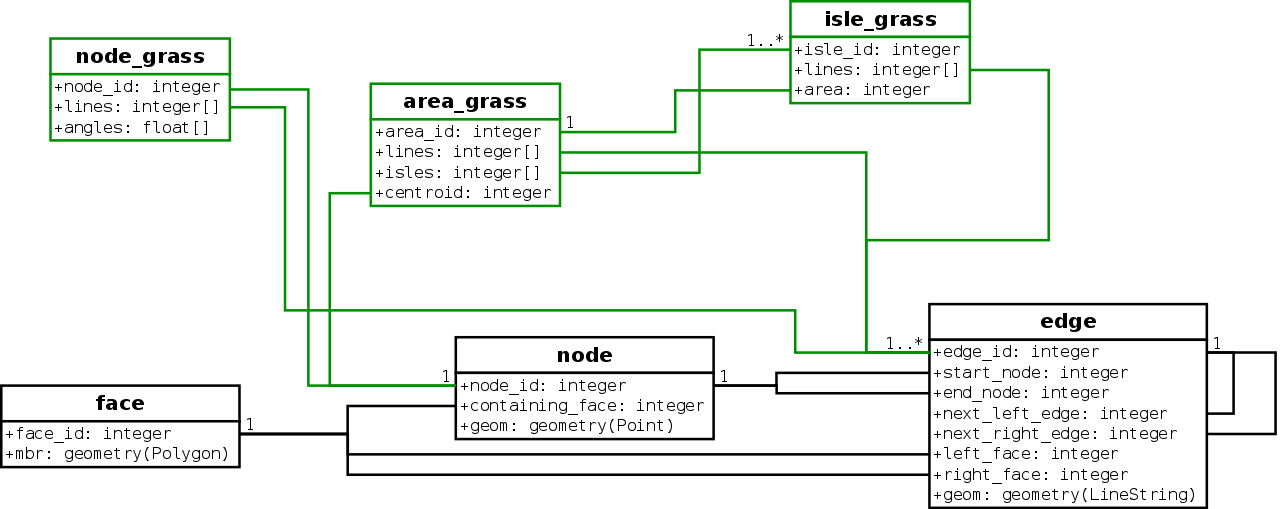
\includegraphics[width=0.47\textwidth]{images/topo-geo-grass}
  \newline
 Figure 3: Extended PostGIS Topology structure
\end{center}

{\bf Dedicated modules}

\begin{itemize}
 \item {\bf v.out.postgis:} Exports a vector map layer to PostGIS feature table.
 \item {\bf v.external:} Creates a new pseudo-vector map as a link to a PostGIS feature table. 
 \item {\bf v.external.out:} Defines vector output format.
\end{itemize}
}



\blocknode{Lidar}{
\smallskip
The Lidar library ({\url {www.liblas.org}}) used by GRASS GIS permits the import of LAS Lidar
data. The imported data can be in raster ({\bf r.in.lidar} using statistics of choice) or in vector format ({\bf v.in.lidar}). \newline
On-farm water storage study with lidar data in NSW (Australia) developed a full remote sensing monitoring methodology
of water availability with lidar-based bathymetric survey and multi-source remote sensing survey [8].\newline
\begin{center}
 %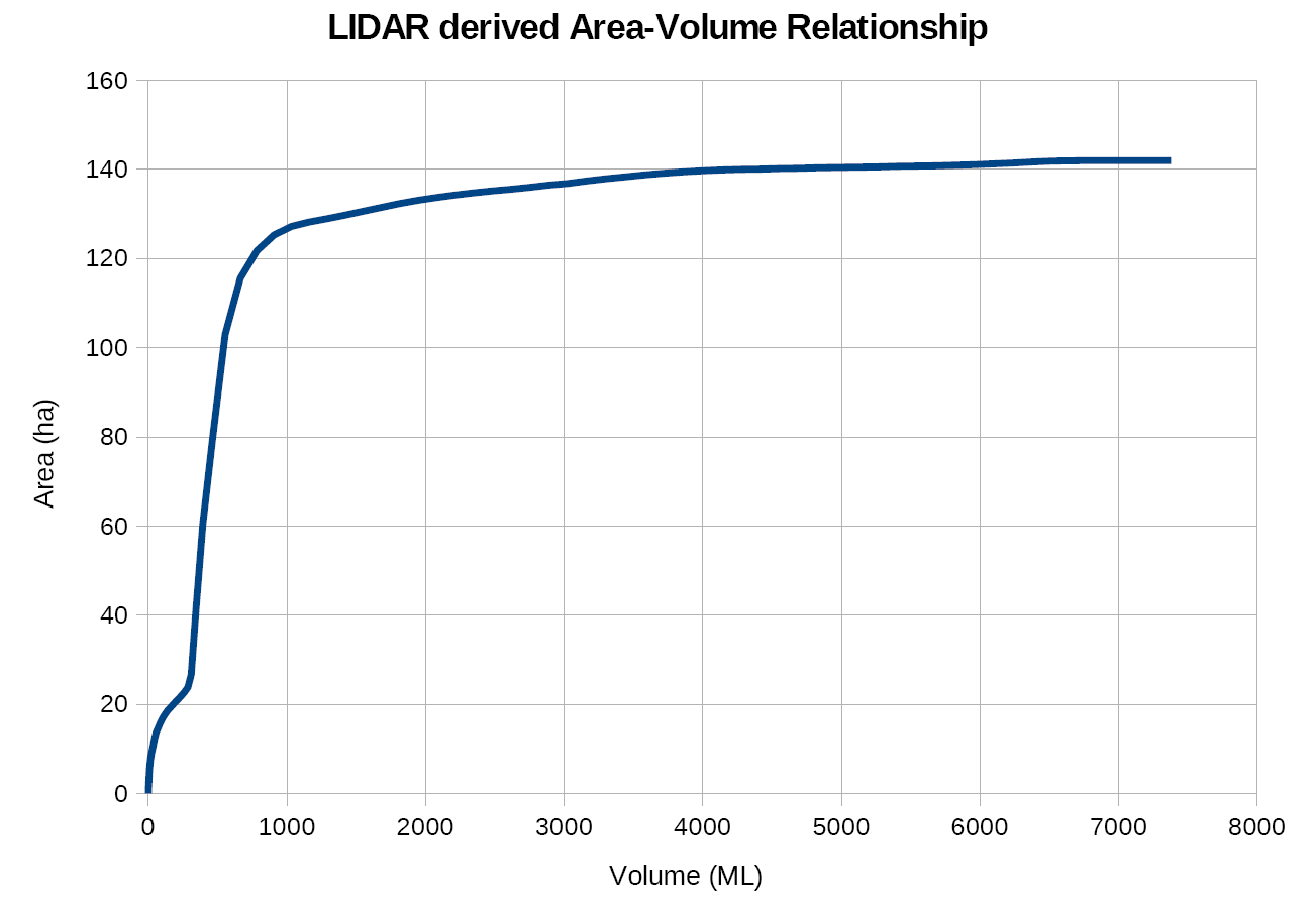
\includegraphics[width=0.4\textwidth]{images/ofs1}
 %\newline
 %Figure 5: On-Farm-Water-Storage Lidar survey and Depth-Volume-Area surveying [8]
 
 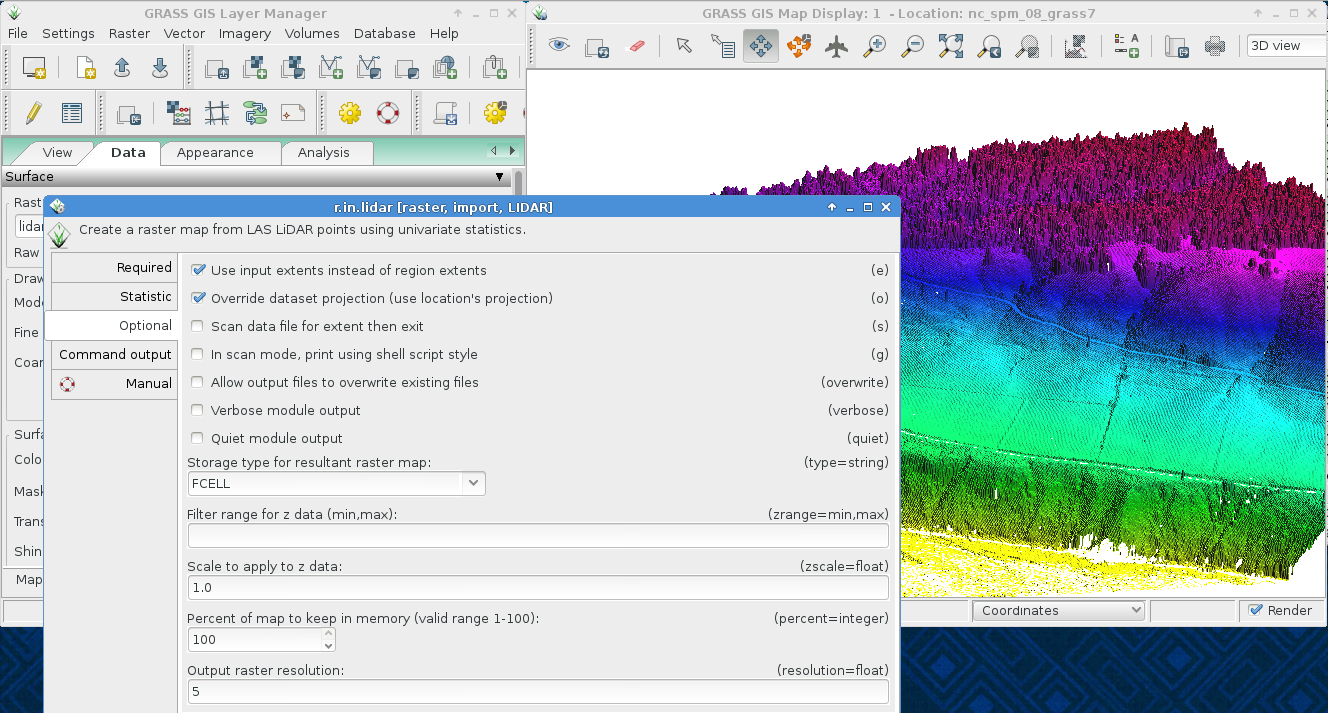
\includegraphics[width=0.4\textwidth]{images/grass7_las_support}
 \newline
 Figure 4: Example for LAS support in GRASS GIS 7: rapid LAS data assessment through binning
\end{center}
}

\blocknode{Other Improvements \& Additions}{
\smallskip

{\bf Remanufacturing, performance improvement}


{\bf Other functions}

\begin{itemize}
 \item {\bf v.distance:} Calculates distances from points, lines, or areas to points, lines, or areas.
 \item {\bf v.overlay:} The processing speed has been substantially improved.
 \item {\bf v.net.*:} All vector network analysis tools provide now fine control over node costs.
 \item {\bf v.voronoi:} New option to create Voronoi diagrams for areas.
 \item {\bf v.rectify:} Vector data can now be georeferenced using various methods for 2D and 3D coordinate transformation.
\end{itemize}
}

\startfourthcolumn
%%%%%%%%%%%%%%%%%%%%%%%%%%%%%%%%%%%%%%%%%%%%%%%%%%%%%%%%%%%%%%%%%%%%%%%%%%%%%%%%
\blocknode{3D}{
\smallskip
Faces

\begin{center}
\begin{tabular}{ll}
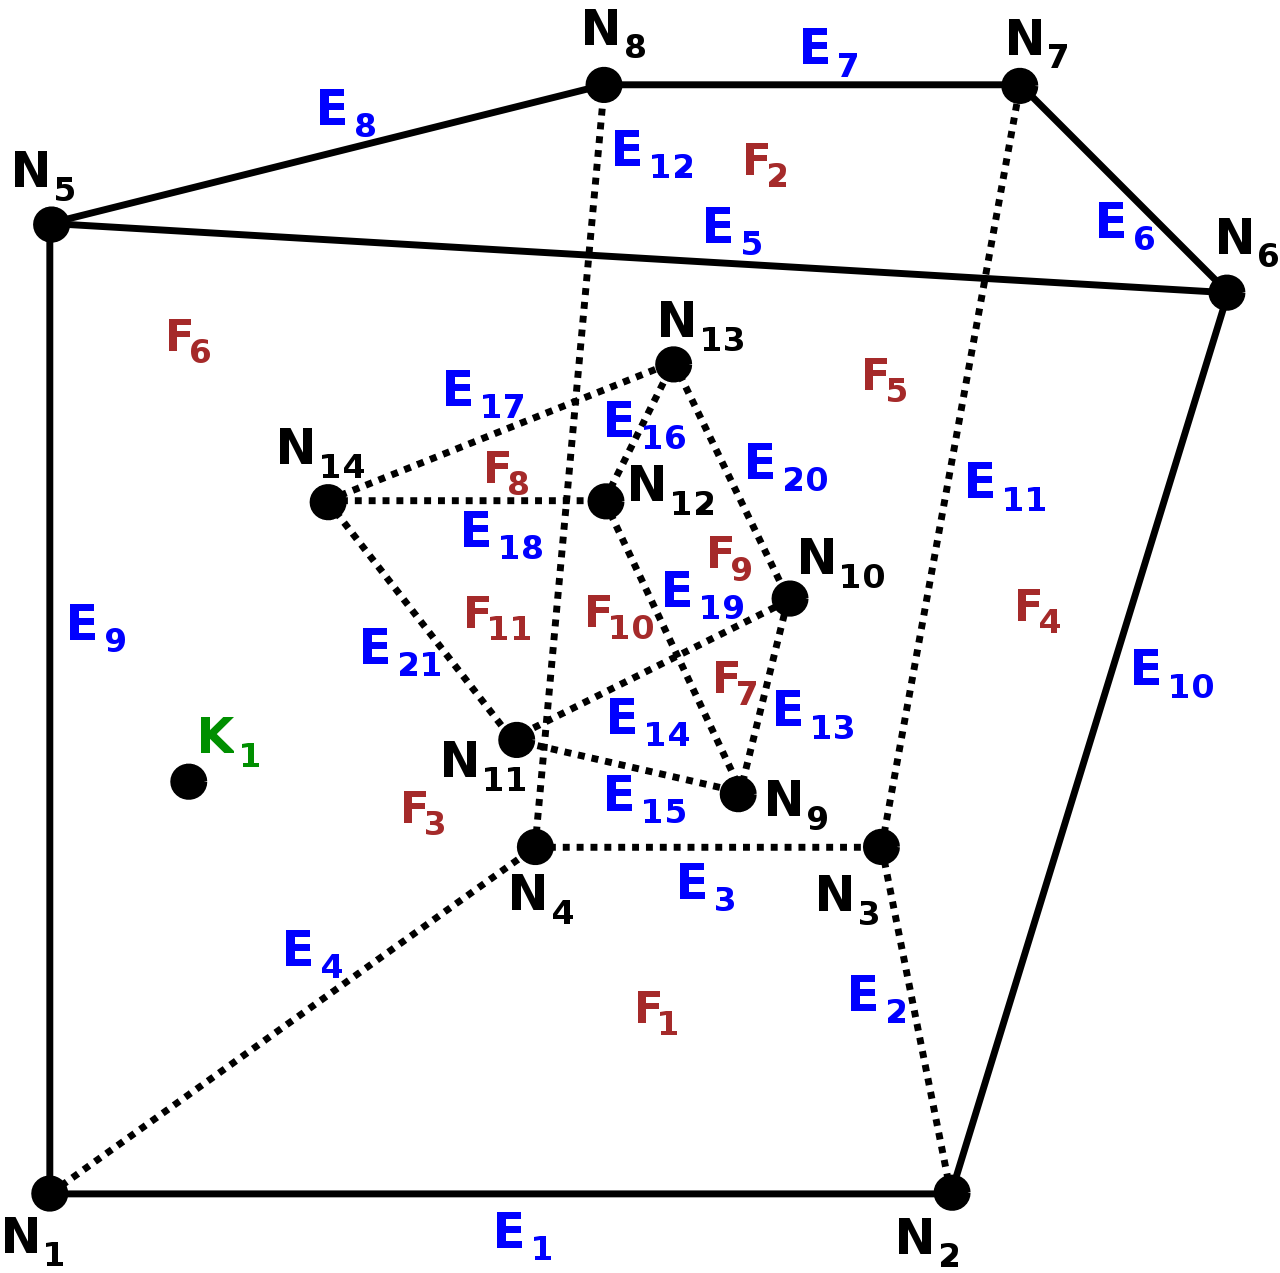
\includegraphics[width=0.30\textwidth]{images/grass7-3d}
& 
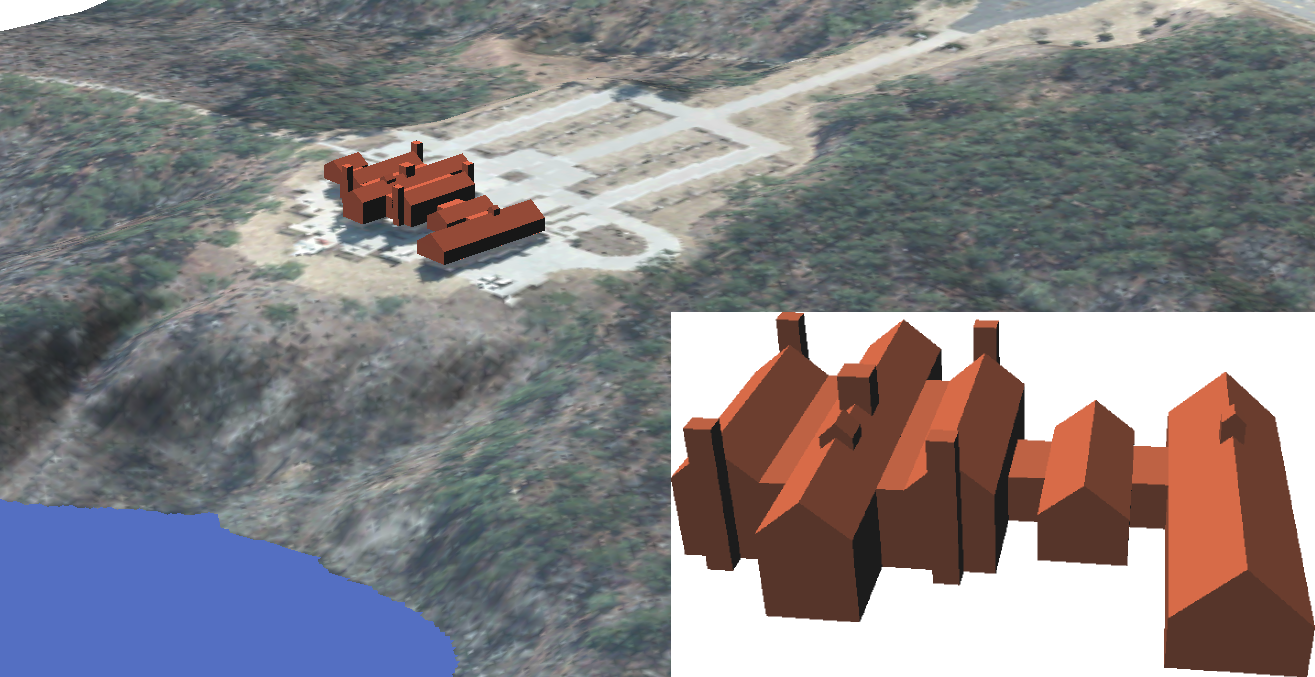
\includegraphics[width=0.55\textwidth]{images/house3D}\\
 Figure 5a: 3D object with a hole &  Figure 5b: 3D model of Chancellor's House (NC State University)\\
 in GRASS GIS topology model& visualized in GRASS GIS
 
\end{tabular}
\end{center}
}

%%%%%%%%%%%%%%%%%%%%%%%%%%%%%%%%%%%%%%%%%%%%%%%%%%%%%%%%%%%%%%%%%%%%%%%%%%%%%%%%

\blocknode{TGRASS: temporal framework}{
TGRASS [Gebbert 2014] provides support for large spatio-temporal data handling and analysis, and is fully integrated into GRASS GIS 7.
It introduces the concept of space-time dataset as a series of vector, raster, or 3D raster data with temporal metadata.
In the simple example below, we computed a series of vector data representing particles in a water flow simulation,
created a space-time dataset and registered the vectors to this dataset based on time stamps assigned during the vector creation.
The result can be then quickly visualized using GRASS GIS Animation Tool.

{\small
\begin{alltt}
r.sim.water -t elevation=elev\_lid792\_1m dx=dx dy=dy depth=depth outwalk=walker outiter=1 

\textcolor{DarkGreen}{t.create} output=particles type=stvds temporaltype=relative semantictype=mean title="Particles"~desc="Particles"

\textcolor{DarkGreen}{t.register} input=particles maps=\textasciigrave g.mlist --q type=vect pattern=walker* separator=,\textasciigrave{} type=vect

g.gui.animation stvds=particles
\end{alltt}}

\begin{center}
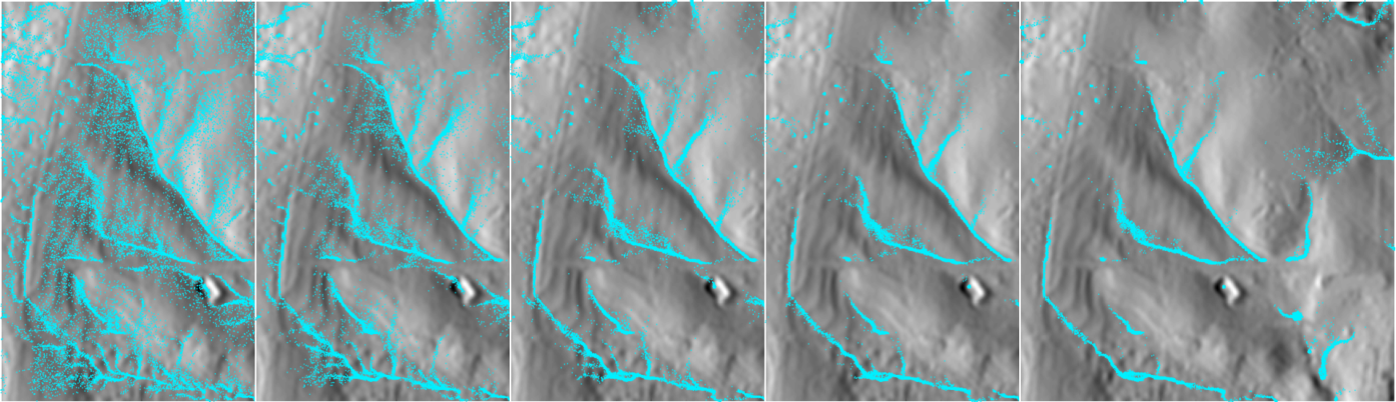
\includegraphics[width=\textwidth]{images/particles}%
\raisebox{0pt}[0pt][0pt]{\hspace{-3cm}\colorbox{white}{
\includegraphics[width=3cm]{images/particles_qr_short}}}%
\newcommand{\seeanimtext}{see animation online}%
\newlength{\myl}%
\settowidth{\myl}{\small\seeanimtext}%
\raisebox{-2ex}[0pt][0pt]{\hspace{-\myl}\colorbox{white}{\small\seeanimtext}}%
\end{center}
}

%%%%%%%%%%%%%%%%%%%%%%%%%%%%%%%%%%%%%%%%%%%%%%%%%%%%%%%%%%%%%%%%%%%%%%%%%%%%%%%%
\blocknode{References}{
% \scriptsize <<- too small for a poster!
\begin{center}
\begin{tabular}{rp{0.8\textwidth}}
[Neteler 2012] & Neteler \& Bowman \&  Landa \& Metz, 2012. Environment \& Modeling Software, 31:124-130\\{}
[Gebbert 2014] & Gebbert \& Pebesma, 2014. TGRASS: A temporal GIS for field based environmental modeling, Environmental Modelling \& Software 53:1–12.\\{}
[Zambelli 2013] & Zambelli \& Gebbert \& Ciolli, 2013. PyGRASS: An Object Oriented Python API for GRASS GIS. ISPRS International Journal of Geo-Information 2.1:201-219.\\{}
[Neteler 2005] & Neteler \& Grasso \& Michelazzi \& Miori \& Merler \& Furlanello, 2005. International Journal of Geoinformatics, 1(1):51-61.\\{}
[Landa 2013] & Landa, 2013. Vektorová architektura systému GRASS GIS [GRASS GIS Vector Architecture]. PhD thesis, CTU in Prague, Czech Republic.
\end{tabular}
\end{center}
\smallskip
\hrulefill
\vspace{-5pt}

\begin{center}
\begin{tabular}{cp{1.9\textwidth}}
\begin{minipage}{0.25\textwidth}

\includegraphics[width=2in]{svg_images/OSGeo_project.pdf}
\end{minipage}

\begin{minipage}{0.3\textwidth}
%\small{\url{www.osgeo.org}}
\url{www.osgeo.org}
\end{minipage}

\begin{minipage}{0.15\textwidth}

\includegraphics[width=1.2in]{images/grass_qr.pdf}
\end{minipage}

\begin{minipage}{0.3\textwidth}
%\small {\url{grass.osgeo.org}}
\url{grass.osgeo.org}
\end{minipage}
\end{tabular}
\end{center}

\hrulefill
\vspace{14pt}
\begin{center}
\newcommand{\logowidth}{5em}
\newcommand{\logospace}{\hspace{0.1em}}
\noindent

\includegraphics[width=\logowidth]{svg_images/public_domain_logo.pdf}
\raisebox{0.7\height}{\logospace 2014 GRASS Development Team}
\end{center}
}

\end{tikzpicture}

\end{document}
